% FILE: sentiment.tex  Version 0.01
% AUTHOR: Uladzimir Sidarenka

% This is a modified version of the file main.tex developed by the
% University Duisburg-Essen, Duisburg, AG Prof. Dr. Günter Törner
% Verena Gondek, Andy Braune, Henning Kerstan Fachbereich Mathematik
% Lotharstr. 65., 47057 Duisburg entstanden im Rahmen des
% DFG-Projektes DissOnlineTutor in Zusammenarbeit mit der
% Humboldt-Universitaet zu Berlin AG Elektronisches Publizieren Joanna
% Rycko und der DNB - Deutsche Nationalbibliothek

\section{Sentiment Corpus}\label{sec:snt:corpus}

A crucial prerequisite for proving or disproving any hypotheses in
computational liguistics is the existence of sufficiently big manually
labeled data for the targeted domain, on which the made conjectures
could be tested.  Since there was no corresponding manually annotated
sentiment corpus for German Twitter that we were aware of at the time
of writing this thesis, we had to create our own dataset, which we
will introduce in this section.

We begin our introduction by describing the selection criteria and
tracking procedure we used to collect the initial raw data for our
``tweebank''.  After detailing the annotation scheme and presenting
the utilized annotation tool, we turn to an extensive analysis of the
inter-annotator agreement, which will serve as an upper bound in our
later experiments.  In Subsection \ref{subsec:snt:iaa}, we propose two
new versions of the popular $\kappa$ metric \cite{Cohen:60} -- binary
and proportional kappa -- which were specifically adjusted to the
peculiarities of our annotation task.  With these two measures, we
estimate the inter-coder reliability of the annotated spans of
subjective opinions, their targets, and sources, also checking whether
the annotators agreed on the polarity and intensity of sentiments and
polar terms, once they agreed on their boundaries.  Finally, with
statistical means, we investigate the correlations between the
selection criteria we applied initially and the number of annotated
elements and disagreements of our experts in the corpus.  That way, we
hope to get a better understanding of which linguistic and
extra-linguistic factors might significantly influence the
distribution of sentiments, and which ones might notably exacerbate
their analysis.

\subsection{Data Collection}

A common question, which typically arises when one starts creating a
new dataset, is that of the selection criteria to use in order to
collect the initial corpus data.  While, for low-level NLP tasks, such
as part-of-speech tagging or syntactic parsing, it typically suffices
to define the language domain to sample from (since the phenomena of
interest are usually frequent and uniformly spread), for semantically
demanding tasks with many diverse ways of expressions, one also has to
pay attention to various in-domain factors as they might considerably
affect the final distribution, making the resulting corpus either
utterly sparse or excessively biased.

To minimize both of these risks -- scarceness and bias -- when
preparing our data, we decided to use a compromise approach by
gathering one part of the new corpus from tweets which were a priori
more likely to contain sentiments, and sampling the rest of the
microblogs from a big collection of messages uniformly at random.  By
doing so, we hoped to increase the recall with the former strategy,
while mitigating the introduced bias with the latter method.

As criteria which could help us find more opinionated microblogs, we
considered the topic and form of tweets.  Our motivation was that some
subjects, such as political or social issues, by themselves could
incite people to be more subjective in their judgements.  Therefore,
including such topics in our corpus would automatically increase the
coverage of sentiments.  On the other hand, opinions also need to be
expressed by some linguistic means, consequently, the mere form of a
message could also suggest whether it was likely to be emotional or
not.

Since we started creating the corpus in the spring 2013, obvious
choices of subjectively rich topics to us were the \emph{papal
  conclave}, which took place in March of that year, and the
\emph{German federal elections}, which were to be held in autumn.
Because both of these events implied some sort of voting, we decided
to include \emph{general discussions of political issues} as another
topic in our dataset in order to counterbalance the election
specifics.  Finally, to obey the second objective, i.e., to keep the
corpus bias low, we considered \emph{casual everyday conversations}
without any pre-defined subjects as the last source of the new data.

In order to collect tweets for the first three topics, we created
extensive keyword lists (with several dozens entries each) for each of
these subjects.  Based on these lists, we subsequently were tracking
microblogs between March and September 2013 using the public Twitter
API.\footnote{\url{https://pypi.python.org/pypi/tweetstream}}
Afterwards, the set of tweets pertaining to the federal elections was
enriched with additional messages, which we obtained from the
University of M\"unster, who were concurrently working on related
problems within the joint FMER project ``Discourse Analysis of Social
Media''.  For sampling the fourth topic, we used the German Twitter
snapshot of \citet{Scheffler:14}, which comprised $\approx97\%$ of
German microblogs posted in April 2013.

This tracking procedure gave us a total of 27.4 M messages with the
M\"unster corpus and Scheffler's collection being by far the most
prolific sources of the data.

%% For our work, the in-domain factors to consider were the topics and
%% the form of tweets.  Since we wanted our corpus to be as
%% representative as possible, we had to make sure that the topics we
%% choose for sampling lend themselves as fruitful opinion sources.  At
%% the same time, we did not want automatically generated ad and news
%% tweets to spoil our data and also introduced additional formal
%% criteria (described below) that the tweets had to satisfy in order to
%% be chosen.  But then again, applying these restriction might make the
%% dataset excessively biased, so we did allow for a certain proportion
%% of tweets being selected even if they did not conform to our
%% constraints.

%% Politics: 59,531 messages, keywords: Altmaier, Wowereit, Minister,
%% Bundeskanzleramt, Schwarz-Gelb

%% Papst: 51,579 messages, keywords: papst, pabst, konklave, Vatikan
%% General Tweets: 51,579 messages, keywords: papst, pabst, konklave, Vatikan

%% Federal Elections: 3,131,315 messages, keywords:

%% General: 24,179,871 messages, keywords:

In the next step, we separated all tweets of the same topic into three
groups based on the following formal criteria:
\begin{itemize}
\item We put messages that contained at least one polar term from the
  sentiment lexicon SentiWS \cite{Remus:10} into the first group;
\item Microblogs which did not satisfy the first condition but
  featured at least one emoticon or exclamation mark were put into the
  second set;
\item Finally, all remaining tweets were allocated to the third formal
  category of their respective topic.
\end{itemize}
With this split, we, again, hoped to increase the recall of sentiments
by separately analyzing messages with already known polar words, which
were also indirectly more likely to contain subjective opinions.  In
order to find such terms, we considered three major German polarity
lists: SentiWS \cite{Remus:10}, German Polarity Clues
\cite{Waltinger:10}, and the Zurich Sentiment Lexicon of
\citet{Clematide:10}, choosing in the end the first one due to its
moderate size, acceptably high precision, and the availability of
inflection forms of its entries.

Since no polar lexicon, however, is guaranteed to provide for the full
coverage of opinionated expressions and, moreover, because Twitter
users are renowned for their creativity in instantly inventing new
language forms \cite{Eisenstein:13}, we also applied a bail-out
approach by separately collecting messages which did not have any
lexicon terms but did contain a smiley or exclamation point.  Our
assumption was that either these elements alone would suffice to
express subjective opinions or that they would reinforce the meaning
of some accidentally missed polar words.

Finally, as we did not make any hypotheses about the distribution of
sentiments in the rest of the tweets, we allocated all remaining
microblogs to the same group, hoping that a uniform sampling from this
set would provide us with further positive and negative opinion
examples.

A detailed breakdown of the resulting distribution of messages across
the four topics and their three formal groups is given in
Table~\ref{snt:tbl:corp:topic-bins}:
\begin{table}[hbt!]\small
  \begin{tabular}{|l|*{5}{>{\centering\arraybackslash}p{0.12\textwidth}|}}
    \hline
    & \multicolumn{4}{c|}{Formal Criterion} & \\\cline{2-5}

    \multirow{-2}{0.2\columnwidth}{\centering\bfseries
      Topic} & Polar Terms
    & Emoticons and Exclamations & Remaining tweets & Total
    &\multirow{-2}{0.12\textwidth}{\centering
      Sample\\ Tracking\\ Keywords}\\\hline

    Federal Elections & 537,083 (22.38\%) & 50,567 (2.1\%) & 1,811,742
    (75.5\%) & 2,399,392 & \tiny\emph{Abgeordnete}
    (\emph{representative}), \emph{Bundesregierung}
    (\emph{federal government})\\\hline

    Papal Conclave & 7,859 (15.11\%) & 1,260 (2.42\%) & 42,879
    (82.46\%) & 51,998 & \tiny\emph{Papst} (\emph{pope}), \emph{Pabst} (\emph{pobe})\\\hline

    Political Discussions & 10,552 (25.8\%) & 777\newline (1.9\%) & 29,555
    (72.29\%) & 40,884 &\tiny\emph{Politik} (\emph{politics}),
    \emph{Minister} (\emph{minister})\\\hline

    General Conversations & 3,201,847 (18.7\%) & 813,478 (4.7\%) &
    13,088,008 (76.5\%) & 17,103,333 & \tiny\emph{den} (\emph{the}),
    \emph{sie} (\emph{she})\\


    \hline
  \end{tabular}
  \caption{Distribution of the downloaded messages across topics and
    formal groups.\newline (percentage numbers are given with respect
    to the total number of tweets pertaining the given
    topic)\label{snt:tbl:corp:topic-bins}}
\end{table}

As can be seen from the table, the vast majority of the tweets in each
topic fall into the third category, i.e., the one where neither polar
terms no common emoticons are present.  The average expected
proportion $\mu$ of such tweets is 76,69\%, and the standard deviation
$\sigma$ from this proportion comes to 4.25\%.  The second biggest
set, whose $\mu$ is equal to 20.5\% and $\sigma$ amounts to $4.62\%$,
is that of microblogs containing emotional terms.  Finally, the group
comprising messages with smileys but supposedly no polar expressions
is the smallest one for each topic.  The expected share of this group
only attains $2.78\%$, deviating by $1.3\%$.

%% Furthermore, as one also can observe, the relative proportions of the
%% formal tweets for the federal elections and political discussions are
%% approximately the same, while general conversations are apparently
%% more biased towards containing polar terms, whereas tweets about the
%% papal conclave, on the contrary, are rather supposed to be objectve.
%% We will check later in Subsection \ref{subsec:snt:iaa} whether the
%% distribution of the annotated sentiments correlates with this
%% proportional split of groups and topics.

In order to generate our final corpus, we eventually chose 666 random
messages from each of the three formal groups of each of the four
subjects, getting a total of 7,992 microblogs: $666\text{ tweets}
\times 4\text{ topics} \times 3\text{ formal criteria}$.  Although
this quota sampling admittedly violates the uniformity principle,
which states that the analyzed instances have to be chosen uniformly
from the whole population, we justify this with the wish to increase
the recall of the phenomena in question and point out to the
possibility of restoring the original distribution parameters by
multiplying the resulting statistics with the proportion coefficients
from Table~\ref{snt:tbl:corp:topic-bins}.

\subsection{Annotation Scheme}\label{subsec:snt:ascheme}
In the next step after collecting the raw data, we defined an
annotation scheme for our corpus. Since our goal was to get a
maximally full coverage of all sentiment-relevant aspects, we devised
an extensive list of elements that had to be annotated by our experts.
This list included:

\begin{itemize}
\item
  \textbf{sentiments}, which we specified as polar subjective
  evaluative opinions about people, subjects, or events.

  According to this definition, three important constraints that a
  potential subjective statement had to satisfy in order to be labeled
  as a sentiment in our dataset were:
  \begin{inparaenum}[\itshape a\upshape)]
  \item \textit{polarity}, i.e., the statement in question had to
    reflect an either positive or negative attitude;
  \item \textit{subjectivity}, i.e., the expressed opinion had to be a
    personal belief not verifiable by any objective means; and,
    finally,
  \item an \textit{evaluative} nature, i.e., the opinionated
    proposition had to refer to some clearly discernable target from
    its surrounding context.
  \end{inparaenum}

  With this element we associated the following types of attributes:
  \begin{itemize}
    \item
      \emph{polarity}, which reflected the attitude of the opinion's
      holder towards the evaluated object.  Following
      \citet{Jindal:06a,Jindal:06b}, we not only distinguished between
      the traditional values for this attribute -- \emph{positive} and
      \emph{negative} -- but also considered \emph{comparison} as a
      separate polarity type, since comparative opinions typically
      only showed relative preferences of the user without implying
      her general fondness or reluctance to any of the juxtaposed
      objects;
    \item
      \emph{intensity}, which showed the emotional strength of the
      expressed sentiment.  Possible values for this property were:
      \emph{weak}, \emph{medium}, and \emph{strong};
    \item
      finally, following \citet{Bosco:13} and \citet{Rosenthal:14}, we
      also explicitly addressed the cases of \emph{sarcasm} by
      providing an eponymous boolean attribute for ironically meant
      comments;
  \end{itemize}

\item
  another element which was closely related to sentiments were
  \textbf{targets}, which we defined as objects or events being
  evaluated by opinion expressions.  For this annotation item, we
  introduced the following three attributes:
  \begin{itemize}
    \item
      the boolean property \emph{preferred}, which was used in
      comparative opinions to distinguish between favored objects and
      the rest of the entities being compared;
    \item
      the link attribute \emph{anaphref}, which was used for
      pronominal targets and had to point to the respective
      antecedents of these proforms (cf. \citet{Stoyanov:06} and
      \citet{Ding:10} on the importance of coreference resolution in
      opinion mining);
    \item
      and, finally, another edge feature -- \emph{sentiment-ref} --
      which was drawn from the target to its respective sentiment in
      cases when the target element was located outside of its opinion
      or on the intersection of two sentiment spans.  This attribute
      had to help us disambiguate the assignment of the evaluated
      objects to their pertaining appraisals when this association was
      not immediately obvious from the context;
  \end{itemize}

\item
  the second crucial component of opinions next to targets were
  \textbf{sources}, which denoted the immediate author(s) or holder(s)
  of evaluative statements.  The only property associated with this
  element was the link attribute \emph{sentiment-ref}, which was
  defined in the same as it was specified for targets.
\end{itemize}

To help our experts identify the text spans of the above elements, we
explicitly defined these entities as \emph{minimal complete syntactic
  or discourse-level units}, i.e., noun phrases or clauses with all
their dependent grammatical and text-level attributes.

A sample tweet annotated according to our definitions is shown in
Example~\ref{snt:exmp:sent-anno1}.

\begin{example}\label{snt:exmp:sent-anno1}
  \upshape\sentiment{\target{Diese Milliardeneinnahmen} sind selbst
    \source{Sch\"auble} peinlich}\\[0.8em]
  \noindent\sentiment{\target{\itshape{}These billions of
      revenue\upshape{}}\itshape{} are embarrassing even for
    \upshape{}\source{\itshape{}Sch\"auble\upshape{}}}
\end{example}

In this sentence, our annotators labeled the complete clause as a
sentiment, since this unit was the minimal syntactic constituent which
simultaneously comprised both the target of the evaluation
(``Milliardeneinnahmen'', \emph{billions of revenue}) and its
respective evaluative expression (``peinlich'', \emph{embarrassing}).
Following our guidelines, the experts also included the complete noun
phrase ``diese Milliardeneinnahmen'' (\emph{these billions of
  revenue}) along with the indefinite pronoun ``diese'' (\emph{these})
into the annotated target span, since the pronoun was syntactically
dependent on the main evaluated term -- ``Milliardeneinnahmen''
(\emph{billions of revenue}).

In addition to the main opinion components (text spans of sentiments,
sources, and targets), our coders also had to label supplementary
elements, which could significantly influence the intensity and
polarity of evaluations.  These elements included:

\begin{itemize}
\item
  \textbf{emotional expressions}, which we defined as lexical items
  (words or idioms) that had a clearly distinguishable polar
  subjective lexical meaning.  Typical examples of such expressions
  were lexemes and set phrases such as ``ekelhaft''
  (\emph{disgusting}), ``lieben'' (\emph{to love}), ``Held''
  (\emph{hero}), ``wie die Pest meiden'' (\emph{to avoid like the
    pest}) etc.

  In contrast to targets and sources, which only could occur in the
  context of an annotated sentiment, emotional expressions were always
  to be marked in text regardless of whether a target-oriented opinion
  was present or not.

  Main attributes of emotional expressions (\emph{polarity},
  \emph{intensity}, and \emph{sarcasm}) largely coincided with the
  attributes defined for sentiments with the only difference that, in
  the case of opinionated terms, the values of these features
  reflected the lexical meaning of the labeled words without taking
  into account their context (i.e., prior polarities and intensities),
  whereas sentiments' attributes showed the compositional meaning of
  the whole opinions (i.e., contextual polarities and intensities of
  evaluations).

  In addition to these common attributes, emotional expressions also
  had element-specific properties: the boolean features
  \emph{subjective-fact} and \emph{uncertain}, and the link attribute
  \emph{sentiment-ref}.  The first property showed whether a polar
  term denoted an objective event with a clear emotional association,
  e.g., ``Atombombe'' (\emph{A-bomb}) or ``Naturschutz''
  (\emph{conservation}).  The second feature was used in the cases
  when the annotators were uncertain about their decisions.  Finally,
  the last attribute was defined in the same way as it was specified
  for targets and sources and had to point from the emotional
  expression to its respective sentiment when an unambiguous
  assignment of the former was impossible;

\item
  elements which increased the expressivity and polar sense of
  opinionated terms were specified as \textbf{intensifiers} in our
  annotation guidelines.  Typical examples of such expressions were
  adverbial modifiers such as ``sehr'' (\emph{very}), ``super''
  (\emph{super}), ``stark'' (\emph{strongly}) etc.;

\item
  \textbf{diminishers}, on the contrary, were words or phrases which
  decreased the polar lexical sense of emotional expressions.
  Similarly to intensifiers, these elements were usually expressed by
  adverbs, e.g., ``weniger'' (\emph{less}), ``kaum'' (\emph{hardly}),
  ``fast'' (\emph{almost}) etc.

  Both of these elements (intensifiers and diminishers) only had two
  types of possible properties: the ordinal feature \emph{degree} with
  two possible values: \emph{medium} and \emph{strong}; and the link
  attribute \emph{emo-expression-ref}, which had to point from the
  modifying element to its pertaining opinionated term;

\item
  the final element -- \textbf{negations} -- was defined as
  grammatical or lexical means which turned the polarity of an
  emotional expression to the complete opposite.  These were typically
  represented by the negative particle ``nicht'' (\emph{not}) or the
  indefinite pronoun ``keine'' (\emph{no}).

  The only attribute associated with this element was the mandatory
  link \emph{emo-expression-ref}, which had to point from the negation
  in question to the opinionated term whose meaning was being
  reversed.
\end{itemize}

In contrast to opinion-level entities, which primarily encompassed
syntactic or discourse-level units, emotional expressions and their
modifiers were explicitly specified as lexical items.  Consequently,
their text spans only had to include single words or discernable
idioms without their possible syntactic adjuncts.

A complete example annotated with both sentiment- and term-level
elements is shown below:
\begin{example}\label{snt:exmp:sent-anno2}
  \tikzstyle{every picture}+=[remember picture]
  \tikzstyle{na} = [shape=rectangle,inner sep=0pt]
  \upshape\sentiment{\target{Die Nazi-Vergangenheit} ist auch
    \negation{\tikz\node[na](word0){nicht};}
    \intensifier{\tikz\node[na](word1){sehr};}
    \emoexpression{\tikz\node[na](word2){r\"uhmlich};}}\\[2.2em]
  \noindent\sentiment{\target{\itshape{}The Nazi
      history\upshape{}}\itshape{} is also
    \negation{\tikz\node[na](word3){not};}
    \upshape{}\intensifier{\tikz\node[na](word4){very};}
    \upshape{}
    \emoexpression{\itshape{}\tikz\node[na](word5){laudable};\upshape{}}}

  \begin{tikzpicture}[overlay]
    \path[->,deeppink4,thick](word0) edge [in=145, out=35] node
         [above] {\tiny emo-expression-ref} (word2);
    \path[->,cyan,thick](word1) edge [in=145, out=30] node
         [above] {\tiny emo-expression-ref} (word2);

    \path[->,deeppink4,thick](word3) edge [in=145, out=35] node
         [above] {\tiny emo-expression-ref} (word5);
    \path[->,cyan,thick](word4) edge [in=145, out=30] node
         [above] {\tiny emo-expression-ref} (word5);
  \end{tikzpicture}
\end{example}
In this case, again, the whole sentence is labeled as a sentiment,
since only the main verb phrase simultaneously comprises both the
target ``Die Nazi-Vergangenheit'' (\emph{The Nazi history}) and its
respective evaluation ``nicht sehr r\"uhmlich'' (\emph{not very
  laudable}).  The boundaries of these two elements -- sentiment and
target -- are determined on the syntactic level, spanning the whole
clause in the former case and encompassing the complete noun phrase
for the latter element.  The polarity attribute of the whole opinion
is set to \emph{negative}, and its intensity is specified as
\emph{medium}.

The emotional expression ``r\"uhmlich'' (\emph{laudable}), its
intensifier ``sehr'' (\emph{very}), and the negation ``nicht''
(\emph{not}), on the contrary, only comprise single words without
their grammatical attributes.  The polarity of the opinionated term is
\emph{positive}, since this is the primarily expressed attitude of
this term disregarding the context.  Both the intensity of the
emotional expression and the degree of its intensifier are set to
\emph{medium}, and the link attribute \emph{emo-expression-ref}
unequivocally shows which opinionated term is being reversed by the
negation and amplified by the intensifying item.\footnote{A more
  detailed description of the annotation elements and their possible
  attributes along with the examples of ambiguous cases can be found
  in the original annotation guidelines provided in
  Appendix~\ref{chap:apdx:sent} of this thesis.}

\subsection{Annotation Tool and Format}\label{subsec:snt:tformat}

For annotating the collected dataset, we used \texttt{MMAX2} -- a
freely available text markup
tool.\footnote{\url{http://mmax2.sourceforge.net/}} The primary
reasons for choosing this program were:
\begin{inparaenum}[\itshape a\upshape)]
 \item its non-commercial license,
 \item the portability to a wide variety of platforms, and
 \item a mature set of annotation features such as possibility to
   create link attributes (used for coreference), mark overlapping
   elements, and assign multiple annotations of the same class to one
   token (which was heavily used by our experts for the cases when one
   sentiment statement was included into another opinion, e.g., ``Sie
   mag diese h\"assliche Jacke'', \emph{She likes this ugly jacket}).
\end{inparaenum}

Since \texttt{MMAX2} relies on a token-oriented stand-off XML format,
where all annotations are stored separately from the original text and
only refer to the ids of the words they are spanning, we first had to
split the downloaded tweets into tokens in order to create an
annotation project\footnote{In \texttt{MMAX2}, an annotation project
  refers to a collection of all XML files pertaining to the same
  corpus, including its text data, annotation files, scheme definition
  etc.} for our data.  To this end, we applied a minimally modified
version of Christopher Potts' social media
tokenizer,\footnote{\url{http://sentiment.christopherpotts.net/code-data/happyfuntokenizing.py}}
which was slightly adjusted to the peculiarities of the German
spelling (we accounted for the capitalized form of German nouns and
the dot at the end of ordinal numbers).

\begin{wrapfigure}{R}{0.5\textwidth}
  \begin{minipage}[t][24.5em]{0.5\textwidth}%
    \hspace{3em}
  \scalebox{0.65}{%
    \begin{minipage}[t][22em]{0.3\textwidth}%
      \small\vspace{-4em}%
      \dirtree{%
        .0 .
        .1 corpus/.
        .2 annotator-1/.
        .2 annotator-2/.
        .4 1.general.mmax.
        .4 ....
        .4 markables/.
        .5 1.general\_diminisher\_level.xml.
        .5 1.general\_emo-expression\_level.xml.
        .5 1.general\_intensifier\_level.xml.
        .5 1.general\_negation\_level.xml.
        .5 1.general\_sentiment\_level.xml.
        .5 1.general\_source\_level.xml.
        .5 1.general\_target\_level.xml.
        .5 ....
        .2 basedata/.
        .3 1.general.words.xml.
        .3 ....
        .2 custom/.
        .3 emo-expression\_customization.xml.
        .3 ....
        .2 scheme/.
        .3 emo-expression\_scheme.xml.
        .3 ....
        .2 source/.
        .3 1.general.xml.
        .3 ....
        .2 style/.
        .1 docs/.
        .2 annotation\_guidelines.pdf.
        .2 ....
        .1 scripts/.
        .2 ....
      }%
    \end{minipage}
  }%
  \end{minipage}

  \begin{minipage}[b]{0.5\textwidth}
  \caption{Directory structure of the sentiment
    corpus.\label{fig:snt:corpus}}%
  \end{minipage}
\end{wrapfigure}

To ease the annotation process and minimize possible data loss during
labeling, we split the complete corpus into 80 smaller project files
with 99 -- 109 tweets each.  In each such file, we put microblogs
pertaining to the same topic, ensuring that the formal groups of that
topic were represented in equal proportions.

In the last preparation step, we finally created the corresponding
scheme and customization settings for the project, which specified
what kinds of elements with which attributes were to be annotated by
the human coders, and how these elements had to look like.

The resulting folder hierarchy of our dataset is shown in Figure
\ref{fig:snt:corpus}.

As can be seen from the listing, the top-level level structure of our
project consists of three main directories:
  \begin{itemize}
  \item\texttt{corpus/}, which includes the actual annotation data;

  \item\texttt{docs/}, in which we placed the annotation guidelines and
    various supplementary documents, such as annotation tests for new
    coders;

  \item and \texttt{scripts/}, which comprises auxiliary scripts for
    estimating the inter-annotator agreement and aligning corpus
    annotations with automatically parsed sentences.
  \end{itemize}

{
  \setlength{\linewidth}{\textwidth}
  The \texttt{corpus/} folder is further subdivided into the
  subdirectories:
  \begin{itemize}
  \item\texttt{annotator-X/}, where X stands for the annotator's id.
    This directory includes the main project files, which specify the
    paths to the annotation directory, tokenization data, appearance
    settings etc.; and the subfolder \texttt{markables/}, which
    comprises the actual annotations;

  \item\texttt{basedata/}, which contains files with tokenized messages;

  \item\texttt{custom/}, which provides customization settings for the
    annotation elements (e.g., their back- and foreground colors, font
    types and size etc.);

    %% {
    %% \setlength{\linewidth}{\textwidth}
  \item\texttt{scheme/}, which includes the definitions of the
    annotation markables,\footnote{In the \texttt{MMAX} terminology, an
      annotation markable is a synonym for an annotation element.}
    their attributes, and possible attributes' values;

  \item\texttt{source/}, where we put the original untokenized
    microblogs;

  \item and, finally, \texttt{style/}, which is the standard
    \texttt{MMAX} directory for storing default settings.
    %% }
  \end{itemize}
}

Examples of an actual annotation file and the underlying tokenization
data are given in Figures \ref{fig:snt:annofile} and
\ref{fig:snt:basefile}.

\begin{minipage}[t]{\textwidth}
  \begin{minipage}[t]{0.45\textwidth}
    \lstset{language=XML}
    \begin{lstlisting}
<?xml version="1.0" encoding="UTF-8"?>
<!DOCTYPE markables SYSTEM "markables.dtd">
<markables xmlns="www.eml.org/NameSpaces/sentiment">
<markable id="markable_259"
span="word_1074..word_1087" sarcasm="false"
mmax_level="sentiment"  polarity="positive"
intensity="medium" />
<markable id="markable_256"
span="word_1056..word_1071" sarcasm="false"
mmax_level="sentiment"  polarity="negative"
intensity="medium" />
<markable id="markable_132"
span="word_1126..word_1139" sarcasm="false"
mmax_level="sentiment"  polarity="positive"
intensity="medium" />
<markable id="markable_70"
span="word_592..word_596" sarcasm="false"
mmax_level="sentiment"  polarity="positive"
intensity="strong" />
...
</markables>
    \end{lstlisting}%
    \captionof{figure}{Example of an annotation file.\label{fig:snt:annofile}}%
  \end{minipage}\hfill%
  %
  \begin{minipage}[t]{0.45\textwidth}%
    \lstset{language=XML}
    \begin{lstlisting}[basicstyle=\tiny]
<?xml version="1.0" encoding="US-ASCII"?>
<!DOCTYPE words SYSTEM "words.dtd">
<words>
<word id="word_1">Gleich</word>
<word id="word_2">in</word>
<word id="word_3">Braunschweig</word>
<word id="word_4">mit</word>
<word id="word_5">Kamaraden</word>
<word id="word_6">Treffen</word>
<word id="word_7">:)</word>
<word id="word_8">EOL</word>
<word id="word_9">@graulich12</word>
<word id="word_10">Das</word>
<word id="word_11">geht</word>
<word id="word_12">ja</word>
<word id="word_13">gar</word>
<word id="word_14">nicht</word>
<word id="word_15">!</word>
...
</words>
    \end{lstlisting}%
    \captionof{figure}{Example of tokenization data.\label{fig:snt:basefile}}%
  \end{minipage}
\end{minipage}

\subsection{Inter-annotator Agreement Metrics}\label{subsec:snt:iaa}

For estimating the inter-annotator agreement (IAA), we adopted the
Cohen's $\kappa$ measure \cite{Cohen:60}.  Following the standard
practice for computing this term as:
\begin{equation*}
  \kappa = \frac{p_o - p_c}{1 - p_c},
\end{equation*}
with $p_o$ denoting the observed agreement and $p_c$ meaning the
agreement by chance, we calculated the observed reliability as the
ratio of tokens with matching annotations to the total number of
tokens:
\begin{equation*}
  p_o = \frac{T - A_1 + M_1 - A_2 + M_2}{T},
\end{equation*}
where $T$ stands for the total token number, $A_1$ and $A_2$ are the
numbers of tokens annotated with the given class by the first and
second annotators respectively, and $M_1$ and $M_2$ represent the
number of tokens with matching annotations for that class.

We also estimated the chance agreement $p_c$ in the usual way as:
\begin{equation*}\textstyle
  p_c = c_1 \times c_2 + (1.0 - c_1) \times (1.0 - c_2),
\end{equation*}
where $c_1$ and $c_2$ are the proportions of tokens annotated with the
given class in the first and second annotations respectively, i.e.,
$c_1 = \frac{A_1}{T}$ and $c_2 = \frac{A_2}{T}$.

Two questions that arose during this computation, however, were
\begin{inparaenum}[\itshape a)\upshape]
  \item whether tokens belonging to several overlapping annotation
    spans of the same class in one annotation had to be counted
    multiple times when computing the $A$ scores (for instance, if we
    had to count the words ``dieses'' (\textit{this}), ``sch\"one''
    (\textit{nice}), and ``Buch'' (\textit{book}) in Example
    \ref{example:snt:iaa} twice as sentiments when computing $A_1$ and
    $A_2$), and
  \item whether we had to assume that two annotated spans from
    different experts agreed on all of their tokens when these spans
    had at least one word in common (e.g., if we had to consider the
    annotation of the token ``Mein'' (\textit{My}) in the following
    example as matching, regarding that the rest of the corresponding
    sentiment spans agreed).
\end{inparaenum}

\begin{example}\label{example:snt:iaa}
\textcolor{red3}{\textbf{Annotation 1:}}\\
\upshape\sentiment{Mein Vater hasst \sentiment{dieses sch\"one Buch}.}\\
\sentiment{\itshape My father hates \upshape\sentiment{\itshape this
    nice book\upshape}.}

\noindent\textcolor{darkslateblue}{\textbf{\itshape Annotation 2:}}\\
Mein \sentiment{Vater hasst \sentiment{dieses sch\"one Buch}.}\\
\itshape My \upshape\sentiment{\itshape{}father hates \upshape\sentiment{\itshape this
    nice book\upshape}.}
\end{example}

To address these issues, we introduced two separate agreement metrics:
\emph{binary} and \emph{proportional} kappa.  With the former variant,
we counted tokens belonging to multiple eponymous annotation spans
multiple times (i.e., $A_1$ and $A_2$ would amount to $10$ and $9$
respectively in the above sample tweet) and considered all tokens
belonging to the given annotation instance as matching if this span
agreed on at least one token with the annotation from the other expert
(i.e., $M_1$ and $M_2$ would have the same values as $A_1$ and $A_2$
in this case).  With the latter metric, every labeled token was
counted only once (i.e., the numbers of the labeled words in the first
and second annotation would correspondingly be equal to $7$ and $6$),
and we only calculated the actual number of tokens with matching
labels when computing the $M$ scores (i.e., both $M_1$ and $M_2$ would
come to $6$ with this metric).  The final values of the binary and
proportional kappa for Example~\ref{example:snt:iaa} would
consequently run up to 1.0 and 0.0 respectively, since the binary
metric would consider both annotations as perfectly matched because
every labeled sentiment instance agreed on at least one token with the
annotation from the other coder, whereas the proportional measure
would stress the fact that the observed agreement $p_o$ was the same
as the agreement by chance $p_c$ and the whole labeling would
therefore be deemed unreliable.

\subsection{Annotation Procedure}\label{sec:astages}
After setting up the agreement metrics, we finally let our experts
annotate the data.  The annotation procedure was carried out in three
steps:
\begin{itemize}
  \item First, both annotators labeled one half of the corpus after
    only minimal training.  Unfortunately, their mutual agreement at
    this stage was relatively low, reaching only 31.21\% for
    sentiments (measured with proportional $\kappa$);
  \item In the second step, in order to improve the inter-rater
    reliability, we automatically determined the differences between
    the two annotations, adding and highlighting unmatched elements as
    a separate class of labelings. We subsequently let our experts
    resolve these discrepancies by either correcting their own
    decisions or rejecting the alternative annotations of the other
    coder.  As in the previous stage, we allowed the annotators to
    consult the supervisor (the author of this thesis) about dealing
    with ambiguous cases, but did not let our assistants communicate
    with each other directly.  This adjudication has lead to
    significant improvements on all annotation levels: The agreement
    on sentiments has improved by 30.73 percentage points, reaching
    61.94\%.  Similar effects were also observed for targets, sources,
    emotional expressions, and their modifiers, resulting in an
    average IAA increase of 25.8 percent;
  \item Finally, after the adjudication was complete, our assistants
    proceeded with the annotation of the remaining files.  Working
    completely independently, one of the experts has annotated 78.8
    percent of the full corpus, whereas the second coder has labeled
    the complete dataset.
\end{itemize}

\subsection{Evaluation}\label{sec:eval}
The agreement results of the initial annotation stage computed with
the two adjusted $\kappa$-metrics are shown in
Table~\ref{tbl:snt:agrmnt-init}.

\begin{table*}[thb!]
  \begin{center}
    \bgroup \setlength\tabcolsep{0.7\tabcolsep} \scriptsize
    \begin{tabular}{|p{0.15\textwidth}| % first columm
        *{10}{>{\centering\arraybackslash}p{0.05\textwidth}|}} % next ten columns
      \hline
          \multirow{2}{0.2\textwidth}{\bfseries Element} &
          \multicolumn{5}{c|}{Binary $\kappa$} & %
          \multicolumn{5}{c|}{Proportional $\kappa$}\\\cline{2-11}
          & $M_1$ & $A_1$ & $M_2$ & $A_2$ & $\mathbf{\kappa}$ %
          & $M_1$ & $A_1$ & $M_2$ & $A_2$ & $\mathbf{\kappa}$\\\hline

          Sentiment & 4,215 & 7,070 & 3,484 & 9,827 & \textbf{38.05} &
          3,269 & 6,812 & 3,269 & 9,796 & \textbf{31.21}\\
          Target & 1,103 & 1,943 & 1,217 & 4,162 & \textbf{35.48} &
          898 & 1,905 & 898 & 4,148 & \textbf{26.85}\\
          Source & 159 & 445 & 156 & 456 & \textbf{34.53} &
          153 & 439 & 153 & 456 & \textbf{33.75}\\
          EExpression & 1,951 & 2,854 & 2,029 & 3,188 & \textbf{64.29} &
          1,902 & 2,851 & 1,902 & 3,180 & \textbf{61.36}\\
          Intensifier & 57 & 101 & 59 & 123 & \textbf{51.71} &
          57 & 101 & 57 & 123 & \textbf{50.81}\\
          Diminisher & 3 & 10 & 3 & 8 & \textbf{33.32} &
          3 & 10 & 3 & 8 & \textbf{33.32}\\
          Negation & 21 & 63 & 21 & 83 & \textbf{28.69} &
          21 & 63 & 21 & 83 & \textbf{28.69}\\\hline
    \end{tabular}
    \egroup
  \end{center}
  \captionof{table}{Inter-annotator agreement after the initial
    annotation stage.\\ {\small ($M1$ -- number of tokens with
      matching labels in the first annotation, $A1$ -- total number of
      tokens labeled with that class in the first annotation, $M2$ --
      number of tokens with matching labels in the second annotation,
      $A2$ -- total number of tokens labeled with that class in the
      second annotation)}}
  \label{tbl:snt:agrmnt-init}
\end{table*}

As can be seen from the table, the inter-rater reliability of
sentiments strongly correlates with the inter-annotator agreement on
targets and sources, setting an upper bound for these elements in the
binary kappa case.  With the proportional metric, however, both
sentiments and targets show inferior results as compared to opinion
holders: the scores for the first two entity types amount to $31.21\%$
and $26.85\%$ respectively, whereas the figures for sources run up to
$33.75\%$.  We explain this difference by the fact, that sentiments
and their targets are typically represented by discourse- or
syntax-level constituents -- clauses or noun phrases -- and, even
though the experts might agree on the presence of these elements more
often (as suggested by the binary measure), reaching a consensus about
the exact boundaries of these items turns out to be a challenging task
despite an explicit clarification of this problem in the guidelines.
Sources, on the other hand, are usually expressed by pronouns, which
rarely accept syntactic attributes and whose boundaries are therefore
easier to determine.  Nevertheless, even with the binary metric, the
agreement figures of all opinion-constituting elements are
significantly below the $40\%$ threshold, which implies only a slight
level of reliability according to the \citeauthor{Landis:77} scale
\cite{Landis:77}.

A different situation is observed for emotional expressions and their
intensifiers though.  The inter-annotator agreement on these elements
is above 60 and 50 percent respectively, for both variants of the
proposed $\kappa$-measure.  Obviously, defining these entities as
lexical units has significantly eased the task of determining their
boundaries.  This effect becomes even more evident when looking at
diminishers and negations, where the $A$ and $M$ token scores are
absolutely identical for both measures.  It means that there was no
single case in the labeled dataset where the annotation spans of these
two elements were overlapping or disagreed on their boundaries once
the annotators were at one about their presence.  Unfortunately, due
to a rather small number of these entities in our corpus -- with only
3 cases of diminishers and 21 cases of negations in total -- the
overall agreement on these elements was relatively small too,
amounting to $33.32\%$ and $28.69\%$.

Since these scores were unacceptable for running further experiments,
we decided to revise diverging annotations by letting our experts
recheck each other's decisions.
%% To this end, we automatically determined conflicting labelings and
%% highlighted them in the annotated \texttt{MMAX2} files.
%% Afterwards, the coders had to decide whether to ignore the
%% highlighted discrepancies or to change ther own decisions.
The results of this adjudication step are shown in
Table~\ref{tbl:snt:agrmnt-adjud}.

\begin{table*}[htb!]
  \begin{center}
    \bgroup \setlength\tabcolsep{0.7\tabcolsep} \scriptsize
    \begin{tabular}{|p{0.15\textwidth}| % first columm
        *{10}{>{\centering\arraybackslash}p{0.05\textwidth}|}} % next ten columns
      \hline
          \multirow{2}{0.2\textwidth}{\bfseries Element} &
          \multicolumn{5}{c|}{Binary $\kappa$} & %
          \multicolumn{5}{c|}{Proportional $\kappa$}\\\cline{2-11}
          & $M_1$ & $A_1$ & $M_2$ & $A_2$ & $\mathbf{\kappa}$ %
          & $M_1$ & $A_1$ & $M_2$ & $A_2$ & $\mathbf{\kappa}$\\\hline

          Sentiment & 8,198 & 8,530 & 8,260 & 14,034 & \textbf{67.92} &
          7,435 & 8,243 & 7,435 & 13,714 & \textbf{61.94}\\

          Target & 3,088 & 3,407 & 2,814 & 5,303 & \textbf{65.66} &
          2,554 & 3,326 & 2,554 & 5,212 & \textbf{57.27}\\

          Source & 573 & 690 & 545 & 837 & \textbf{72.91} &
          539 & 676 & 539 & 833 & \textbf{71.12}\\

          EExpression & 3,164 & 3,298 & 3,261 & 4,134 & \textbf{85.68} &
          3,097 & 3,290 & 3,097 & 4,121 & \textbf{82.64}\\

          Intensifier & 111 & 219 & 113 & 180 & \textbf{56.01} &
          111 & 219 & 111 & 180 & \textbf{55.51}\\

          Diminisher & 9 & 16 & 10 & 16 & \textbf{59.37} &
          9 & 16 & 9 & 15 & \textbf{58.05}\\

          Negation & 68 & 84 & 67 & 140 & \textbf{60.21} &
          67 & 83 & 67 & 140 & \textbf{60.03}\\\hline
    \end{tabular}
    \egroup
  \end{center}
  \captionof{table}{Inter-annotator agreement after the adjudication
    step.\\ {\small ($M1$ -- number of tokens with matching labels in
      the first annotation, $A1$ -- total number of labeled tokens in
      the first annotation, $M2$ -- number of tokens with matching
      labels in the second annotation, $A2$ -- total number of labeled
      tokens in the second annotation)}}
  \label{tbl:snt:agrmnt-adjud}
\end{table*}

As can be seen from the figures, this procedure has significantly
improved the inter-rater reliability on all annotation levels: the
binary scores of sentiments and targets have increased by $29.87\%$
and $30.18\%$ respectively.  An even greater improvement occurs for
sources, whose binary kappa has risen by remarkable $38.38\%$.  A
similar tendency can be observed in terms of the proportional metric:
here, the agreement on sentiments has gained 30.73 percentage points,
reaching $61.94\%$.  Likewise, the reliability of opinion subjects and
holders has improved by $30.42\%$ and $37.37\%$, running up to $57.27$
and $71.12$ percent respectively.

In general, however, we can see that the second annotator tended to
label almost twice as many sentiment and target elements as the first
expert: the proportional $A_1$ scores of these two entity types come
to 8,243 and 3,326 tokens, whereas the corresponding $A_2$ figures
amount up to 13,714 and 5,212 words.  A better consistency in this
regard is achieved on sources, where the number of the labeled items
in both annotations differs only by a factor of 1.2.

As in the previous step, the highest agreement scores are attained by
emotional expressions, whose reliability significantly surpasses the
80\% benchmark, achievening an almost perfect level.  Interestingly
enough, only 193 out of 3,290 opinionated terms annotated by the first
expert did not match the labelings of the second coder, who again
tended to mark generally more elements than the first assistant.
Another notable observation is that the difference between the binary
and proportional scores of the emotional expressions only runs up to
3.04\%, which suggests that the assistants could unproblematically
determine the boundaries of these terms in most of the cases.

Somewhat surprisingly, the agreement improvement on intensifiers was
notably smaller than the reliability increases obtained for sentiments
and polar terms.  The resulting figures of the intensifying elements
were, in fact, even worse than the scores attained by other modifiers
-- diminishers and negations, even though the opposite situation was
seen after the first annotation run.  A closer look at the diverging
cases revealed that the majority of these disagreements stemmed from a
different treatment of exclamation marks: the first expert had been
skipping these entities during the annotation, whereas the second
coder had regarded them as valid intensifying expressions.
Nevertheless, even despite these diverging interpretations, the
reliability on intensifiers was above the $55\%$ threshold, reaching a
moderate agreement.

After ensuring that our annotators could reach an acceptable quality
of coding, we finally let them label the remaining part of the data.
The agreement results of this stage computed on the files annotated by
both experts are given in Table~\ref{tbl:snt:agrmnt-final}.

\begin{table*}[thb!]
  \begin{center}
    \bgroup \setlength\tabcolsep{0.7\tabcolsep} \scriptsize
    \begin{tabular}{|p{0.15\textwidth}| % first columm
        *{10}{>{\centering\arraybackslash}p{0.05\textwidth}|}} % next ten columns
      \hline
          \multirow{2}{0.2\textwidth}{\bfseries Element} &
          \multicolumn{5}{c|}{Binary $\kappa$} & %
          \multicolumn{5}{c|}{Proportional $\kappa$}\\\cline{2-11}
          & $M_1$ & $A_1$ & $M_2$ & $A_2$ & $\mathbf{\kappa}$ %
          & $M_1$ & $A_1$ & $M_2$ & $A_2$ & $\mathbf{\kappa}$\\\hline

          Sentiment & 14,748 & 15,929 & 14,969 & 26,047 & \textbf{65.03} &
          13,316 & 15,375 & 13,316 & 25,352 & \textbf{58.82}\\

          Target & 5,765 & 6,629 & 5,292 & 9,852 & \textbf{64.76} &
          4,789 & 6,462 & 4,789 & 9,659 & \textbf{56.61}\\

          Source & 966 & 1,207 & 910 & 1,619 & \textbf{65.99} &
          898 & 1,180 & 898 & 1,604 & \textbf{64.1}\\

          EExpression & 5,574 & 5,989 & 5,659 & 7,419 & \textbf{82.83} &
          5,441 & 5,977 & 5,441 & 7,395 & \textbf{80.29}\\

          Intensifier & 192 & 432 & 194 & 338 & \textbf{49.97} & 192 &
          432 & 192 & 338 & \textbf{49.71}\\

          Diminisher & 16 & 30 & 17 & 34 & \textbf{51.55} & 16 & 30 &
          16 & 33 & \textbf{50.78}\\

          Negation & 111 & 132 & 110 & 243 & \textbf{58.87} & 110 &
          131 & 110 & 242 & \textbf{58.92}\\\hline
    \end{tabular}
    \egroup
  \end{center}
  \captionof{table}{Inter-annotator agreement of the final
    corpus.\\ {\small ($M1$ -- number of tokens with matching labels
      in the first annotation, $A1$ -- total number of labeled tokens
      in the first annotation, $M2$ -- number of tokens with matching
      labels in the second annotation, $A2$ -- total number of labeled
      tokens in the second annotation)}}
  \label{tbl:snt:agrmnt-final}
\end{table*}

This time, we can observe a slight decrease of the results: the
proportional score for sentiments drops by $3.12\%$, whereas the
agreement figures for targets stay more persistent and lose only 0.66
percent, going down from $57.27\%$ to $56.61\%$.  The most dramatic
changes occur for sources, whose proportional value deteriorates by
notable $7.02$ percentage points, sinking to $64.1\%$.  Nonetheless,
the average proportional agreement of all these elements is around 60
percent, which is almost twice as high as the mean reliability
achieved after the first step.

As before, the scores of emotional expressions are in the ballpark of
almost perfect results \cite[cf.][]{Landis:77}.  Their modifying
elements, however, show a decrease: the agreement on intensifiers
deteriorates by 5.8\% to 49.71\% proportional kappa.  A similar
situation is observed for diminishers, whose $\kappa$-rank worsens
from $58.05\%$ to $50.78\%$.  The best persistence in this regard is
shown by negations, where the quality drops only by $1.11\%$, which
can be considered as a very good result, regarding the generally small
number of these elements in our corpus.

In general, we can see that the reliability of all elements in the
final dataset is at least moderate, with emotional expressions being
the most dependably labeled items ($\kappa_{\textrm{p}}=80.29\%$) and
intensifiers setting the lower boundary of the agreement scores
($\kappa_{\textrm{p}}=49.71\%$).

In order to understand the reasons for the remaining disagreements, we
turned to a qualitative inspection of diverging annotations in our
corpus.  A sample sentence with different analyses of sentiments is
shown below:
\begin{example}\label{snt:exmp:sent-disagr}
  \textcolor{red3}{\textbf{Annotation 1:}}\\ \upshape{}@TinaPannes
  immerhin ist die \#afd nicht dabei \smiley{}\\[0.8em]\itshape
  \noindent\textcolor{darkslateblue}{\textbf{\itshape Annotation
      2:}}\\ \upshape{}@TinaPannes
  \sentiment{\textcolor{red}{immerhin ist die \#afd nicht
      dabei \smiley{}}}\\[0.8em]
  \noindent\itshape{}@TinaPannes
  \upshape\sentiment{\textcolor{red}{\itshape{}anyway the \#afd is
      not there \smiley{}}\upshape{}}
\end{example}
As can be seen from the labels, the first coder erroneously overlooked
the emoticon \smiley{} at the end of the tweet, whereas the second
expert correctly recognized this smiley as an evaluation of the
content set forth in the preceding clause.  Since our annotators had
different opinions about the presence of a sentiment in this
microblog, they trivially disagreed on the annotation of the target
element too, which, in this case, was the verb phrase ``immerhin ist
die \#afd nicht dabei'' (\emph{anyway the \#afd is not there}).

At this point, we should note that it also was possible to consider
the noun phrase ``die \#afd'' (\emph{the \#afd}) as the object of the
evaluation in this message.  We, however, advised the assistants to be
as specific as possible when determining the targets of the
opinions. So, if a sentiment was related to a particular action
performed by an agent (which, in this case, was the fact of afd's
being somewhere) rather than the agent herself, they better had to
label the complete verb phrase and not only its acting subject.  With
this rule, we hoped to better distinguish targets in sentences like
``die Partei hat das Gesetz verabschiedet \smiley{}'' (\emph{the party
  has adopted this law \smiley{}}) from the objects of evaluations in
microblogs like ``die Partei hat das Gesetz abgelehnt \smiley{}''
(\emph{the party has rejected this law \smiley{}}), which were clearly
describing two completely different events so that labeling similar
targets, e.g., ``die Partei'' (\emph{the party}), in both of these
messages would be unequivocally wrong in that case.

A much rarer case of diverging target annotations occurred when the
experts actually agreed on the sentiment spans.  An example of such
situation is shown in the following tweet:
\begin{example}\label{snt:exmp:targt-disagr}
  \textcolor{red3}{\textbf{Annotation
      1:}}\\
  \upshape{}\sentiment{Koalition wirft der SPD
    \target{\textcolor{red}{Blockadehaltung}} vor}\\[0.5em]
  \noindent\itshape{}\sentiment{Coalition accuses the SPD of
    \target{\textcolor{red}{blocking politics}}}\\[0.6em]\itshape

  \noindent\textcolor{darkslateblue}{\textbf{\itshape Annotation
      2:}}\\
  \upshape{}\sentiment{Koalition wirft \target{\textcolor{red}{der SPD}}
    Blockadehaltung vor}\\[0.5em]
  \noindent\itshape{}\sentiment{Coalition accuses
    \target{\textcolor{red}{the SPD}} of blocking politics}
\end{example}

In this sentence, the first coder considered the reproached fact of
the \emph{blocking politics} as the object of the evaluation, whereas
the second expert regarded the political party being accused of such
behavior as the target of the sentiment.  In our opinion, both of
these options were valid in this case and, ideally, two sentiment
elements had to be labeled in this message: one with the target
``Blockadehaltung'' (\emph{blocking politics}) and another one with
the target ``die SPD'' (\emph{the SPD}).

Even though our assistants were much more consistent when labeling
emotional expressions than when analyzing opinion-level entities, we
decided to have a look at diverging annotations of these entities too,
in order to understand the difficulties in the remaining conflicts.  A
sample case of diverging interpretations of polar terms is shown in
Example~\ref{snt:exmp:emo-disagr}

\begin{example}\label{snt:exmp:emo-disagr}
  \textcolor{red3}{\textbf{Annotation 1:}}\\ \upshape{}Syrien vor dem
  Angriff -- bringen diese Bomben den Frieden?\\[0.3em]\itshape
  \noindent\itshape{}Syria facing an attack -- will these bombs bring
  peace?\\

  \noindent\textcolor{darkslateblue}{\textbf{\itshape Annotation
      2:}}\\ \upshape{}Syrien vor dem
  \emoexpression{\textcolor{red}{Angriff}} -- bringen diese
  \emoexpression{\textcolor{red}{Bomben}} den
  \emoexpression{\textcolor{red}{Frieden}}?\\[0.3em]
  \noindent\itshape{}Syria facing an
  \upshape\emoexpression{\textcolor{red}{\itshape{}attack}\upshape}\itshape{}
  -- will these
  \upshape\emoexpression{\textcolor{red}{\itshape{}bombs}\upshape}\itshape{}
  bring
  \upshape\emoexpression{\textcolor{red}{\itshape{}peace}\upshape}\itshape{}?
\end{example}

Apparently, in this sentence, the renowned subjective facts were the
primary source of annotators' confusion: the first coder has skipped
the words ``Angriff'' (\emph{attack}), ``Bombe'' (\emph{bomb}), and
``Frieden'' (\emph{peace}), whereas the second expert has regarded
these tokens as valid opinionated items.  Even though our original
guidelines were underspecified in this case (we only imposed the
subjectivity constraint on sentiments), in our later experiments
(cf.~Section~\ref{sec:snt:lex}), labeling these terms turned out to be
a better solution when comparing the corpus annotation with the
existing sentiment lexica.

In addition, we should note that these different takes of subjective
facts were to some extent due to the adjudication procedure that we
applied in step two of the annotation: a closer analysis of these
cases revealed that, at the initial stage, our experts had had
opposite preferences regarding subjective facts (viz., the first
annotator had typically annotated them, whereas the second coder had
usually skipped these words).  During the revision, however, both
assistants interpreted their decisions as false, and both changed
their minds.  Even though the rest of their changes made in that step
has still lead to significant improvements, the possibility of mutual
concessions needs to be kept in mind when applying the adjudication
method in future.

In order to see whether our experts also agreed on the attributes of
the items they labeled, we additionally computed the Cohen's $\kappa$-
and Krippendorff's $\alpha$-metrics \cite{Krippendorff:07} on the
polarities and intensities of matching sentiments and emotional
expressions.  The reason for choosing two different measures to assess
the annotation quality of these features was that the polarity was a
binary attribute, for which we only needed to estimate the number of
cases where its values were equal -- therefore, we applied the
$\kappa$-coefficient to estimate its reliability.  Intensity, on the
other hand, was a categorial trait whose values were ranging from zero
(weak) to two (strong).  Since disagreements which were far apart on
the scale were to be penalized more than near divergencies, we opted
for the Krippendorff's $\alpha$-metric as it by default allowed for
such distinctions.  The results of these computations are shown in
Table~\ref{tbl:attr-agrmnt}.

\begin{table}[thb!]
  \begin{center}
    \bgroup \setlength\tabcolsep{0.47\tabcolsep} \scriptsize
    \begin{tabular}{|p{0.23\columnwidth}|%
          *{2}{>{\centering\arraybackslash}p{0.2\columnwidth}|}} % next five columns
      \hline
          {\bfseries Element} & Polarity $\kappa$ & Intensity $\alpha$\\\hline
          Sentiment & 58.8 & 73.54\\
          EExpression & 87.12 & 78.79\\
          \hline
    \end{tabular}
    \egroup
    \caption{Inter-annotator agreement on polarity and intensity of
      sentiments and emotional expressions.}
    \label{tbl:attr-agrmnt}
  \end{center}
\end{table}

As can be seen from the scores, reaching a consensus about the
polarities of emotional terms was a much easier task than agreeing on
the value of this attribute for complete sentiments.  Similar to
Example~\ref{snt:exmp:sent-disagr}, one of the main reasons for these
disagreements were subjective opinions containing smileys, especially
in cases when the polarity of the emoticon contradicted the polarity
of its preceding sentence, e.g., ``Ich hasse die Piratenpartei
\smiley{}'' (\emph{I hate the Pirate Party {\upshape \smiley{}}}).

Interestingly enough, the ordinal inter-rater agreement on the
intensities of sentiments ($\alpha = 73.54$) is notably higher than
the corresponding figures for the binary reliability of their
polarities ($\kappa = 58.8$).  The opposite situation is observed for
the emotional expressions though: the $\alpha$-value for the
intensities of these items ($78.79$) is almost ten percent lower than
the corresponding $\kappa$-results for their binary polarities
(87.12).

For the sake of completeness, we also compared these figures with the
scores obtained on the MPQA corpus \cite[cf.][pp. 38, 80]{Wilson:07}.
The average $\alpha$-agreement on the intensity of direct subjective
and objective speech events (a rough counterpart of our sentiments) on
this dataset was around 79\%.  The corresponding results for the
intensity of expressive subjective elements (emotional expressions in
our case) were much worse though, only amounting to 46\%, even though
the respective $\kappa$-value of their polarity attained considerable
72\%.  It means that the reliability results of our corpus
outperformed all but the sentiment intensity scores of MPQA.  We
should, however, note that the annotation scheme used for this dataset
did not provide a specific attribute for the polarity of sentiments,
but specified the polarity of opinionated terms as their contextual
valence, i.e., the polarity of the respective term with its possible
modifications from the surrounding context.

Finally, in order to check how the selection criteria that we applied
initially for sampling our corpus affected the resulting distribution
of sentiments and polar expressions in the resulting dataset, we
generated statistics plots on the frequencies and agreement level of
these elements in our data
(cf. Figures~\ref{snt:fig:crp-sent-emo-distr}
and~\ref{snt:fig:crp-sent-emo-agr}).

\begin{figure*}[htbp!]
{
\centering
\begin{subfigure}{.5\textwidth}
  \centering
  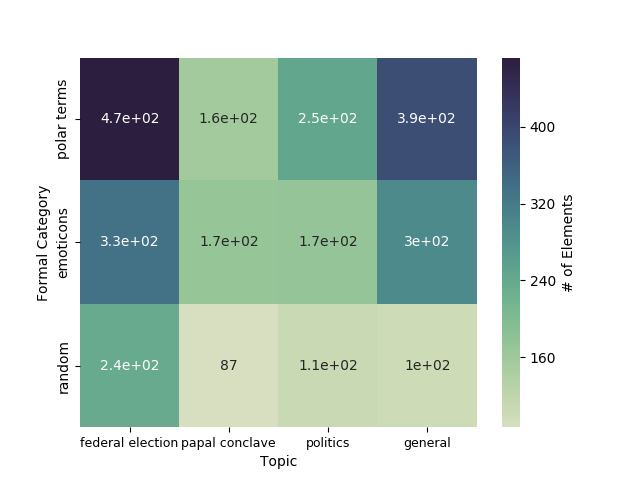
\includegraphics[width=\linewidth]{img/sentiment_stat.png}
  \caption{\texttt{Sentiments}}\label{snt:fig:crp-sent-emo-distr-a}
\end{subfigure}%
\begin{subfigure}{.5\textwidth}
  \centering
  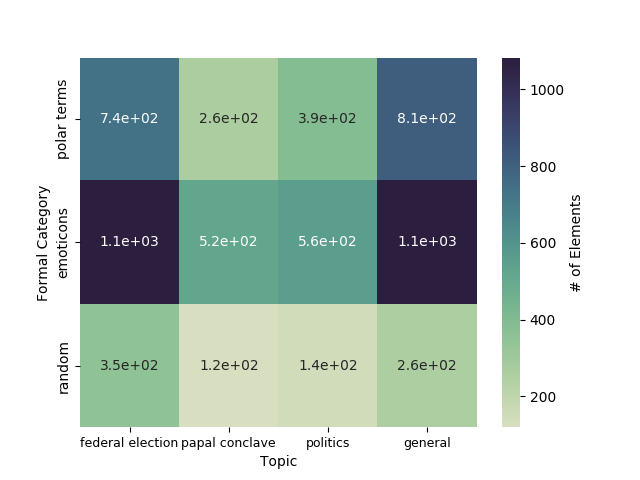
\includegraphics[width=\linewidth]{img/emo-expression_stat.png}
  \caption{\texttt{Emotional expressions}}\label{snt:fig:crp-sent-emo-distr-b}
\end{subfigure}
}
\caption{Distribution of sentiments and emotional expressions across
  topics and formal categories.}\label{snt:fig:crp-sent-emo-distr}
\end{figure*}

\begin{figure*}[htbp!]
{
\centering
\begin{subfigure}{.5\textwidth}
  \centering
  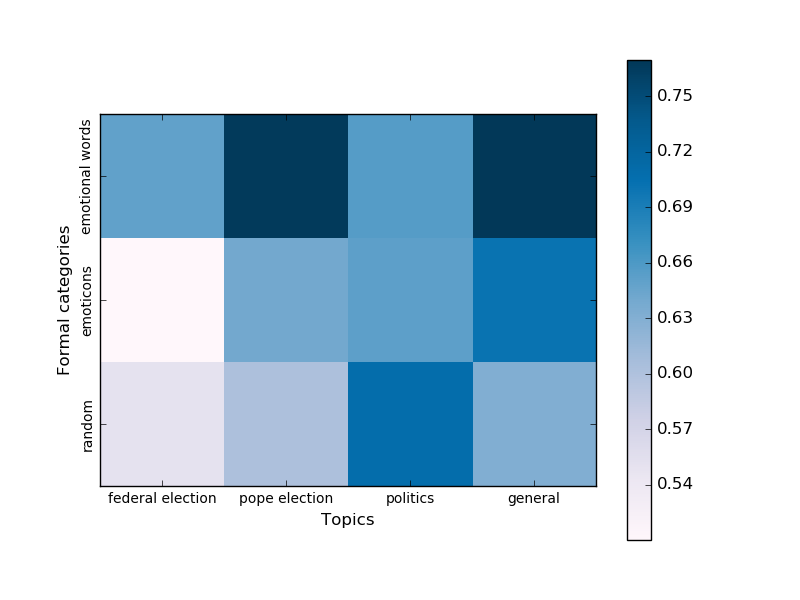
\includegraphics[width=\linewidth]{img/sentiment_agreement.png}
  \caption{\texttt{Sentiments}}
\end{subfigure}%
\begin{subfigure}{.5\textwidth}
  \centering
  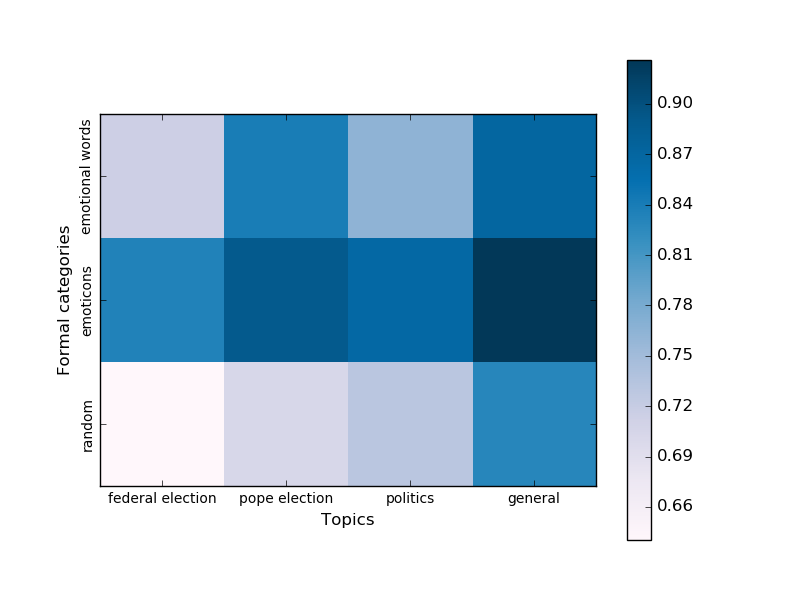
\includegraphics[width=\linewidth]{img/emo-expression_agreement.png}
  \caption{\texttt{Emotional expressions}}
\end{subfigure}
}
\caption{Inter-annotator agreement on sentiments and emotional
  expressions across topics and formal categories.}\label{snt:fig:crp-sent-emo-agr}
\end{figure*}

As can be seen from the results, the stratification according to the
topics and formal traits of the downloaded messages has notably
influenced both the number of these elements and the difficulty of
their interpretation.  According to
Figure~\ref{snt:fig:crp-sent-emo-distr}, federal elections and
topically unfiltered tweets are the ones with the highest number of
annotated opinions.  A similar tendency is also observed for emotional
expressions, although, in this case, the formal grouping appears to
play a more important role than the topics.  Somewhat surprisingly,
the higher number of opinionated terms does not necessarily lead to a
higher number of targeted sentiments.  We can recognize that from the
fact that, even though the biggest number of subjective opinions
appear in the first row of Plot~\ref{snt:fig:crp-sent-emo-distr-a}
(i.e., in tweets with terms from the SentiWS lexicon), most of the
polar terms show up in row two of
Plot~\ref{snt:fig:crp-sent-emo-distr-b} (i.e., in microblogs
containing smileys).

As to the inter-annotator agreement, we can see that the highest
reliability of the annotated opinions is achieved on general tweets
taken from casual everyday conversations.  This message group is also
the one with the highest IAA scores for emotional expressions.  The
formal grouping, however, seems to behave differently in this case:
here, the first category (i.e., tweets with known lexicon terms)
appears to comprise messages with the most reliably annotated
sentiments, whereas the second group (i.e., messages containing
emoticons) is the easiest one for annotating polar lexical items.
Surprisingly, this group is among the most difficult ones for
analyzing complete opinions, which suggests that, even though, smileys
are commonly recognized as emotional expressions, the question whether
these expressions relate to something particular in the tweet or
rather denote the general mood of the author might often be difficult
to answer.

To confirm these observations (viz., the correlation between the
topics and formal groups of the tweets on the one hand and the number
and reliability of sentiments and emotional expressions on the other),
we have also computed the correlation coefficients ($\rho$) of these
parameters.  The results of these computations are shown in
Table~\ref{sent:tbl:corr-coeff}.
\begin{table}[thb!]
  \begin{center}
    \bgroup \setlength\tabcolsep{0.47\tabcolsep} \scriptsize
    \begin{tabular}{|p{0.2\columnwidth}|%
          *{4}{>{\centering\arraybackslash}p{0.18\columnwidth}|}} % next five columns
      \hline

      & \multicolumn{4}{c|}{\bfseries Correlation Coefficients}\\\cline{2-5}

      & \multicolumn{2}{c|}{Sentiment}& %
      \multicolumn{2}{c|}{Emotional Expression}\\\cline{2-5}

      \multirow{-3}{0.2\columnwidth}{\centering\bfseries Selection Criteria} & %
      \# of elements & agreement & \# of elements & agreement\\\hline

      \multicolumn{5}{|c|}{\cellcolor{cellcolor}Topical Groups}\\\hline
      Federal Elections & \textbf{0.312} & 0.169 & 0.356 & 0.289\\
      Papal Conclave & 0.149 & 0.124 & 0.182 & 0.264\\
      Political Discussions & 0.195 & 0.148 & 0.218 & 0.244\\
      General Conversations & 0.183 & \textbf{0.19} & \textbf{0.372} & \textbf{0.452}\\\hline
      \multicolumn{5}{|c|}{\cellcolor{cellcolor}Formal Categories}\\\hline
      Polar Terms & \textbf{0.445} & \textbf{0.352} & 0.38 & 0.301\\
      Emoticons & 0.127 & 0.096 & \textbf{0.47} & \textbf{0.615}\\
      Random & 0.216 & 0.134 & 0.143 & 0.138\\
      \hline
    \end{tabular}
    \egroup
    \caption{Correlation coefficients of topics and formal selection
      criteria with the number and reliability scores of sentiments
      and emotional expressions.}
    \label{sent:tbl:corr-coeff}
  \end{center}
\end{table}

As can be seen from the figures, both topical and formal criteria show
positive correlations with the number of annotated elements and
inter-annotator agreement thereon.  The only possible explanation for
this is that the phenomena which cause difficulties to the experts are
evenly spread among those groups rather than being concentrated in one
place.

As to particular $\rho$-scores, we can see that the strongest
correlation with the number of sentiments is achieved by the federal
elections and polar terms groups, where it amounts to 0.312 and 0.445
respectively.  Topics, however, seem to have a much smaller impact on
the agreement on these elements: the maximum $\rho$-value here is
attained by the general conversations category and only comes up to
0.19 points.  Polar terms, on the other hand, show a much stronger
influence, reaching a correlation coefficient of 0.352.

A slightly different situation is observed for the emotional
expressions: the highest scores for this element both in terms of the
number of annotated items and their reliability are achieved by the
general conversations and emoticons groups.  As to the number of
labeled instances, the $\rho$-coefficients of these two corpus parts
run up to 0.372 and 0.47 respectively.  The impact of these groups on
the agreement appears to be even stronger as the correlation values
reach remarkable 0.452 and 0.615 points.

In general, we can say that, to a greater or lesser extent, virtually
every annotation aspect of the resulting corpus except for the
sentiment agreement is correlated with the topic or form of the tweets
being analyzed.  As to the reliability of sentiments, we hypothesize
that the mere task of recognizing subjective opinions in microblogs
was so challenging for the human experts (which was also confirmed by
our initial annotation experiments) that the difficulties with
interpreting the guidelines instructions and applying these
instructions to concrete cases were playing a much more crucial role
and posed much bigger problems to the coders than the particular
specifics of topical and formal groups.

Notwithstanding the last finding, the agreement scores achieved in the
last stage and the rest of the statstics presented in this chapter
suggest that our assistants could eventually agree not only on the
boundaries of sentiment elements but also on the text spans of their
pertaining sources and targets as well as pertaining opinionated
terms.  Furthermore, the results shown in Table~\ref{tbl:attr-agrmnt}
prove that the polarity and intensity attributes of these elements
could be dependably analyzed either.  Last but not least, the
statistics plots on the distribution of subjective opinions and
emotional expressions show how different sampling criteria have
affected the final composition and agreement level of the corpus.

\subsection{Related Work}

\subsection{Summary and Conclusion}

\newpage
